\section{Auswertung}
\label{sec:Auswertung}
\subsection{Bestimmung der Schallgeschwindigkeit}
Aus \eqref{??}[$\lambda$ abhängig von d] kann die Schallgeschwindigkeit über die Differenz der Resonanzfrequenzen
bestimmt werden. Hierfür werden diese gegen die Länge der Röhren aufgetragen. Die Länge der Röhren ist bekannt, da immer Röhren 
der gleichen Länge hinzugefühgt werden.
\FloatBarrier
\begin{table}
    \centering
    \caption{Messwerte für die Bestimmung der Schallgeschwindigkeit}
    \label{tab:Schallgeschwindigkeit}
    \begin{tabular}{c c c c}
        \toprule
        Länge /\SI{}{\milli\meter}& erste Resonanz /\SI{}{\kilo\hertz} & zweite Resonanz /\SI{}{\kilo\hertz}& Differenz /\SI{}{\kilo\hertz}\\
        \midrule
        $\num{50}$&$\num{6.87}$&$\num{10.28}$&$\num{3.41}$\\
        $\num{100}$&$\num{6.89}$&$\num{8.6}$&$\num{1.71}$\\
        $\num{150}$&$\num{6.895}$&$\num{8.05}$&$\num{1.16}$\\
        $\num{200}$&$\num{6.897}$&$\num{7.759}$&$\num{0.86}$\\
        $\num{250}$&$\num{6.9}$&$\num{7.59}$&$\num{0.69}$\\
        $\num{300}$&$\num{6.9}$&$\num{7.477}$&$\num{0.58}$\\
        \bottomrule
    \end{tabular}
\end{table}
\FloatBarrier
Durch die Messwerte aus \ref{tab:Schallgeschwindigkeit} wird die Funktion
\begin{equation*}
    f(x) = a \frac{1}{x} + b
\end{equation*}
gefittet.\\
Mit der Gleichung 
\begin{equation*}
    nc = 2df +b =2a+b
\end{equation*}
kann die Schallgeschwindigkeit bestimmt werden.
\FloatBarrier
\begin{figure}
    \caption{Messwerte und Fitfunktion für die Bestimmung der Schallgeschwindigkeit}
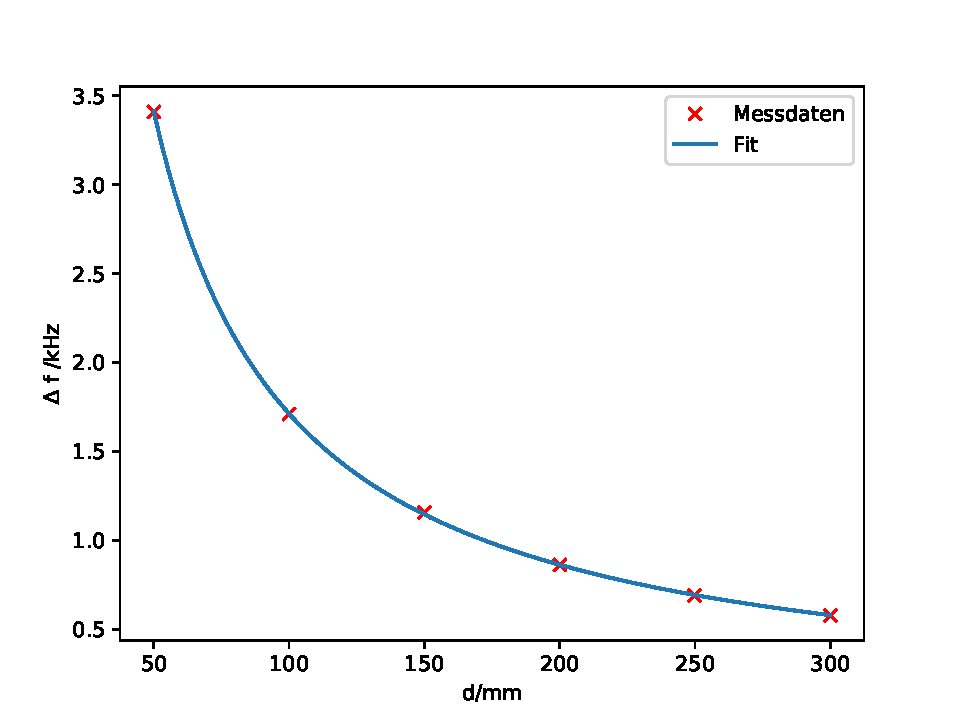
\includegraphics[width = \textwidth]{figure/Schallgeschwindigkeit.pdf}
\end{figure}
\FloatBarrier
Die Parameter der Funktion sind:
\begin{equation*}
    a= \num{169.9(3)}\\
    b= \num{0.013(3)}
\end{equation*}
Daraus kann der Wert $c=\SI{339.8(7)}{\meter\per\second}$ bestimmt werden.

\subsection{Wasserstoffatom}
Als vorbereitenden Versuch für diese Messreihe, wird das Frequenzspektrum auf zwei verschiedene Arten vermessen.
Anschließend werden die Methoden verglichen.
